%! Author = heged
%! Date = 2023. 02. 14.

% Preamble
\documentclass{article}

% Packages
\usepackage{graphicx}
\usepackage{blindtext}
\usepackage[normalem]{ulem}
\usepackage{hyperref}
\usepackage{listings}
\usepackage[cache=false]{minted}
% Document
\title{Ora2}
\author{Hegedüs János}
\date{February 2023}
\begin{document}
    \maketitle
    \selection{Introduction}
    \blindtext[4]
    \begin{figure}[h]
        \centering
        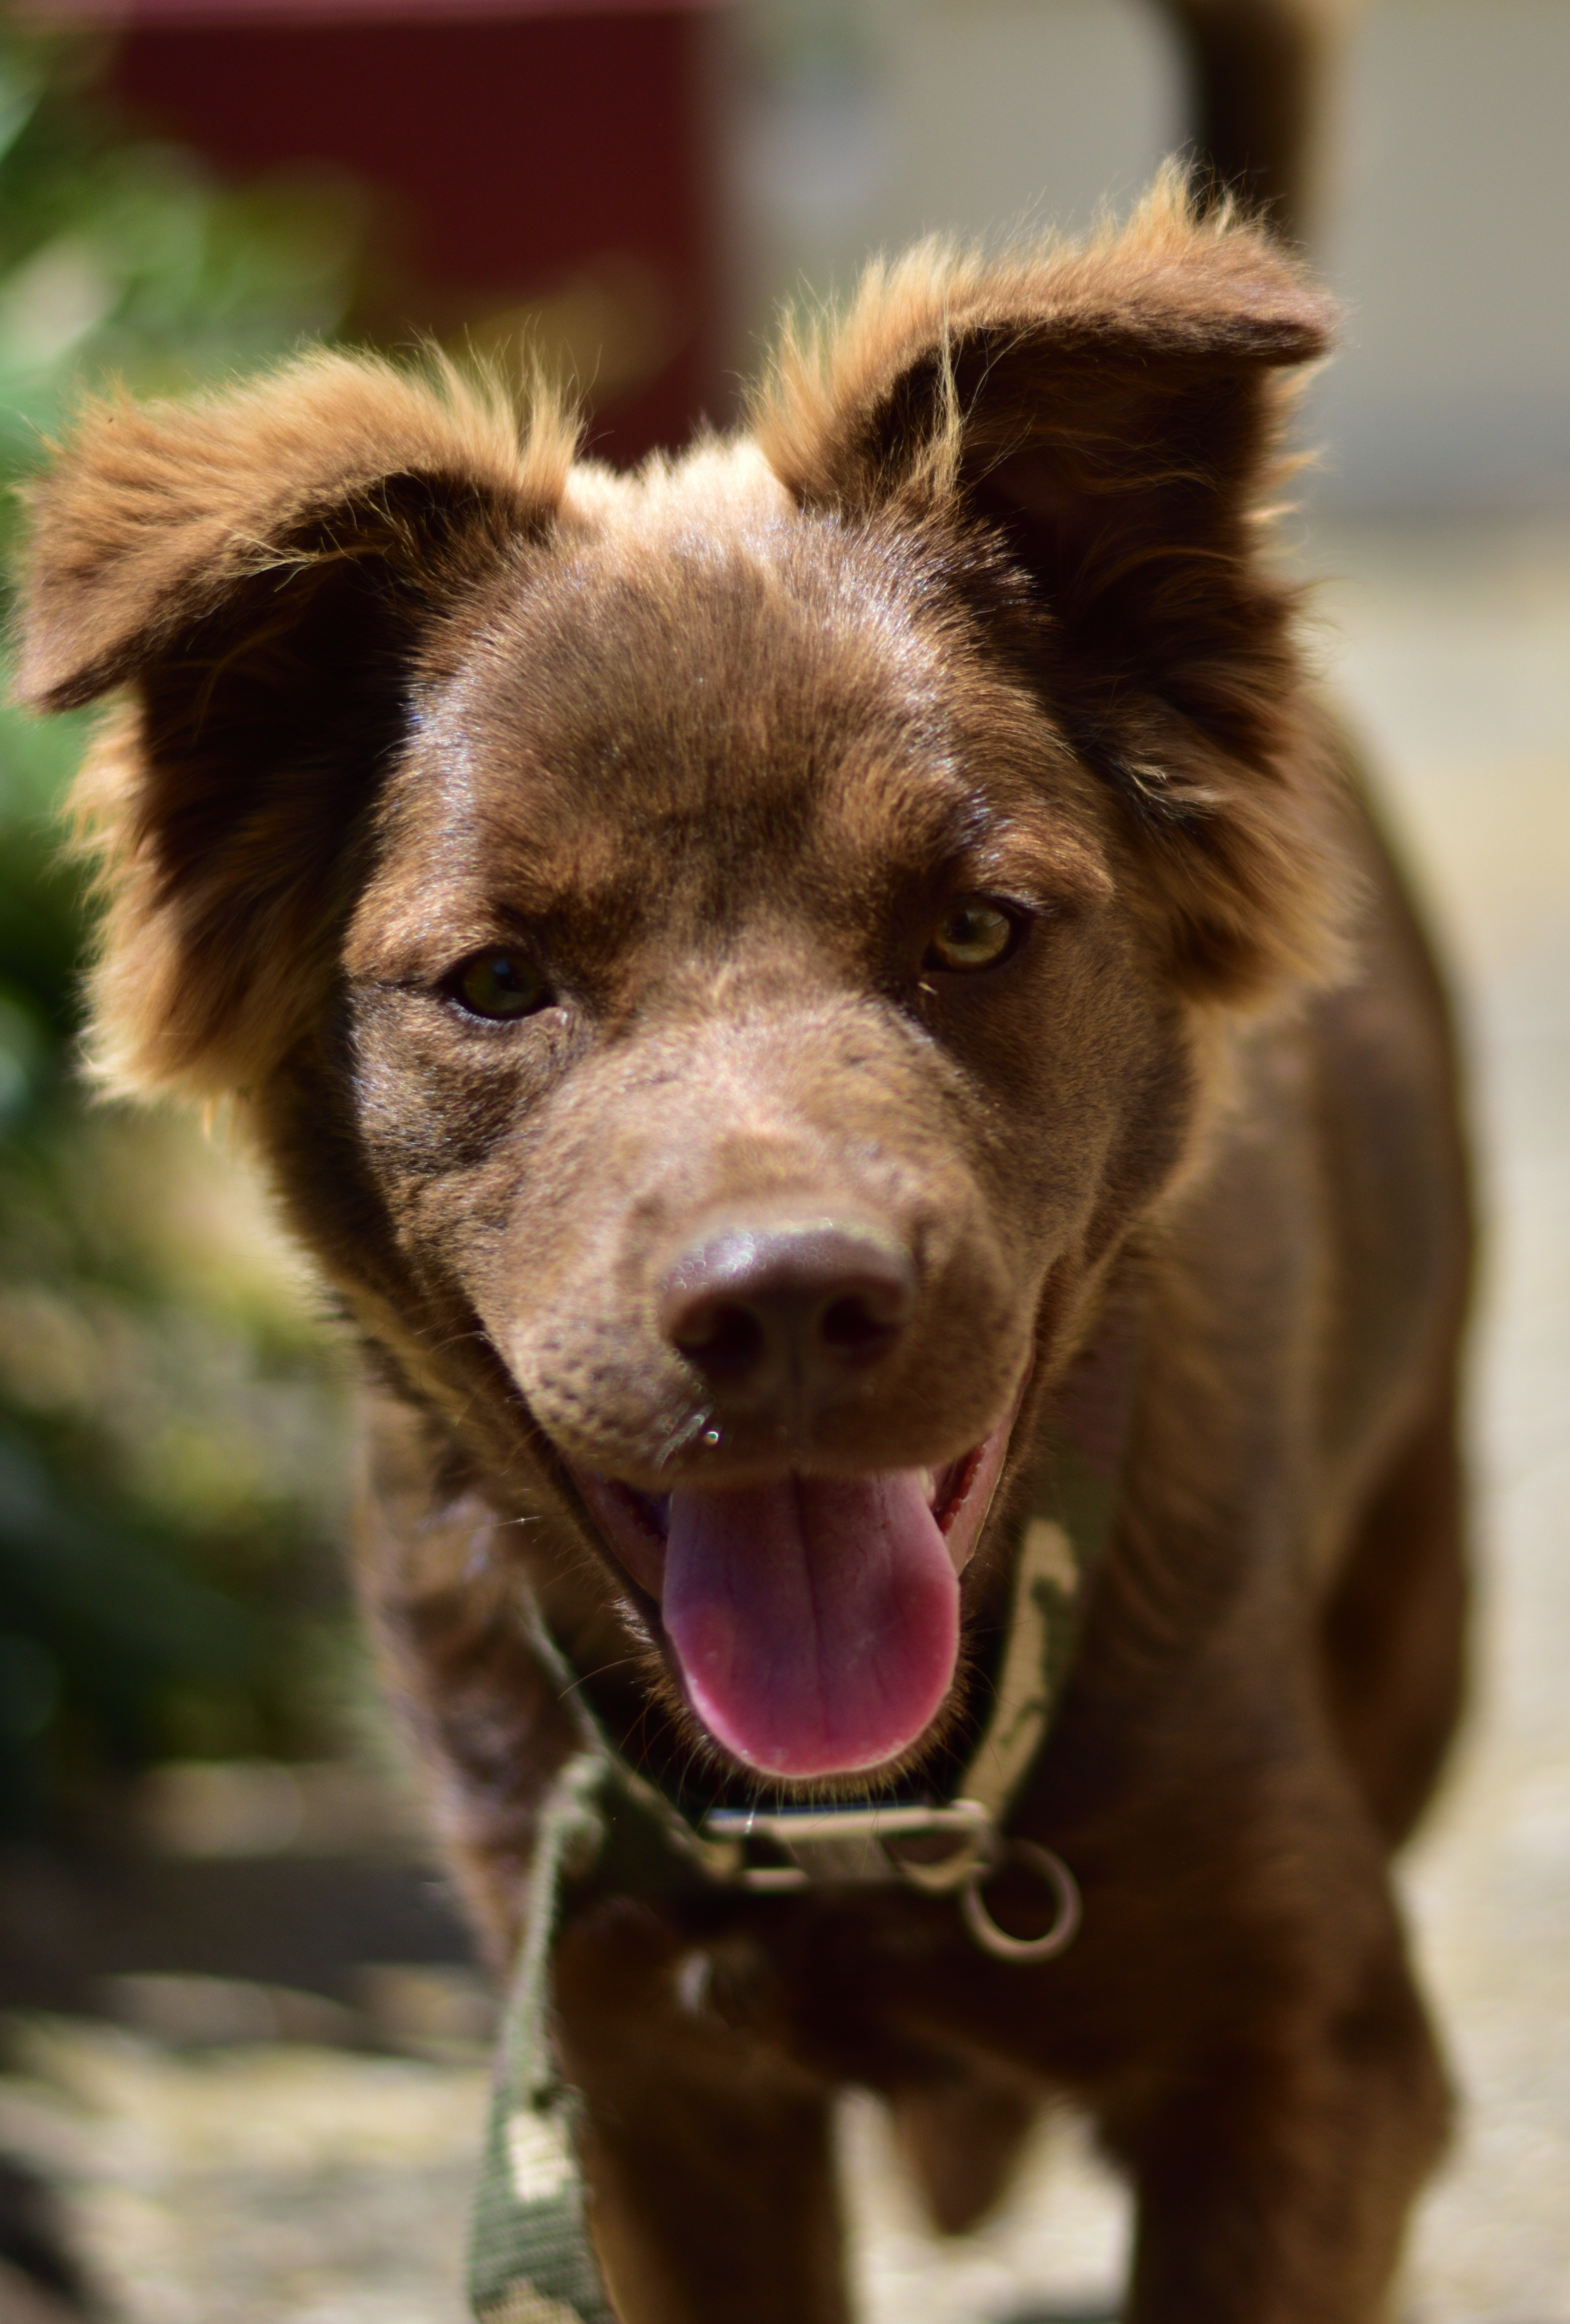
\includegraphics[width=0.5\textwidth]{resources/kep}
    \end{figure}
    \begin{figure}[p]
        \centering
        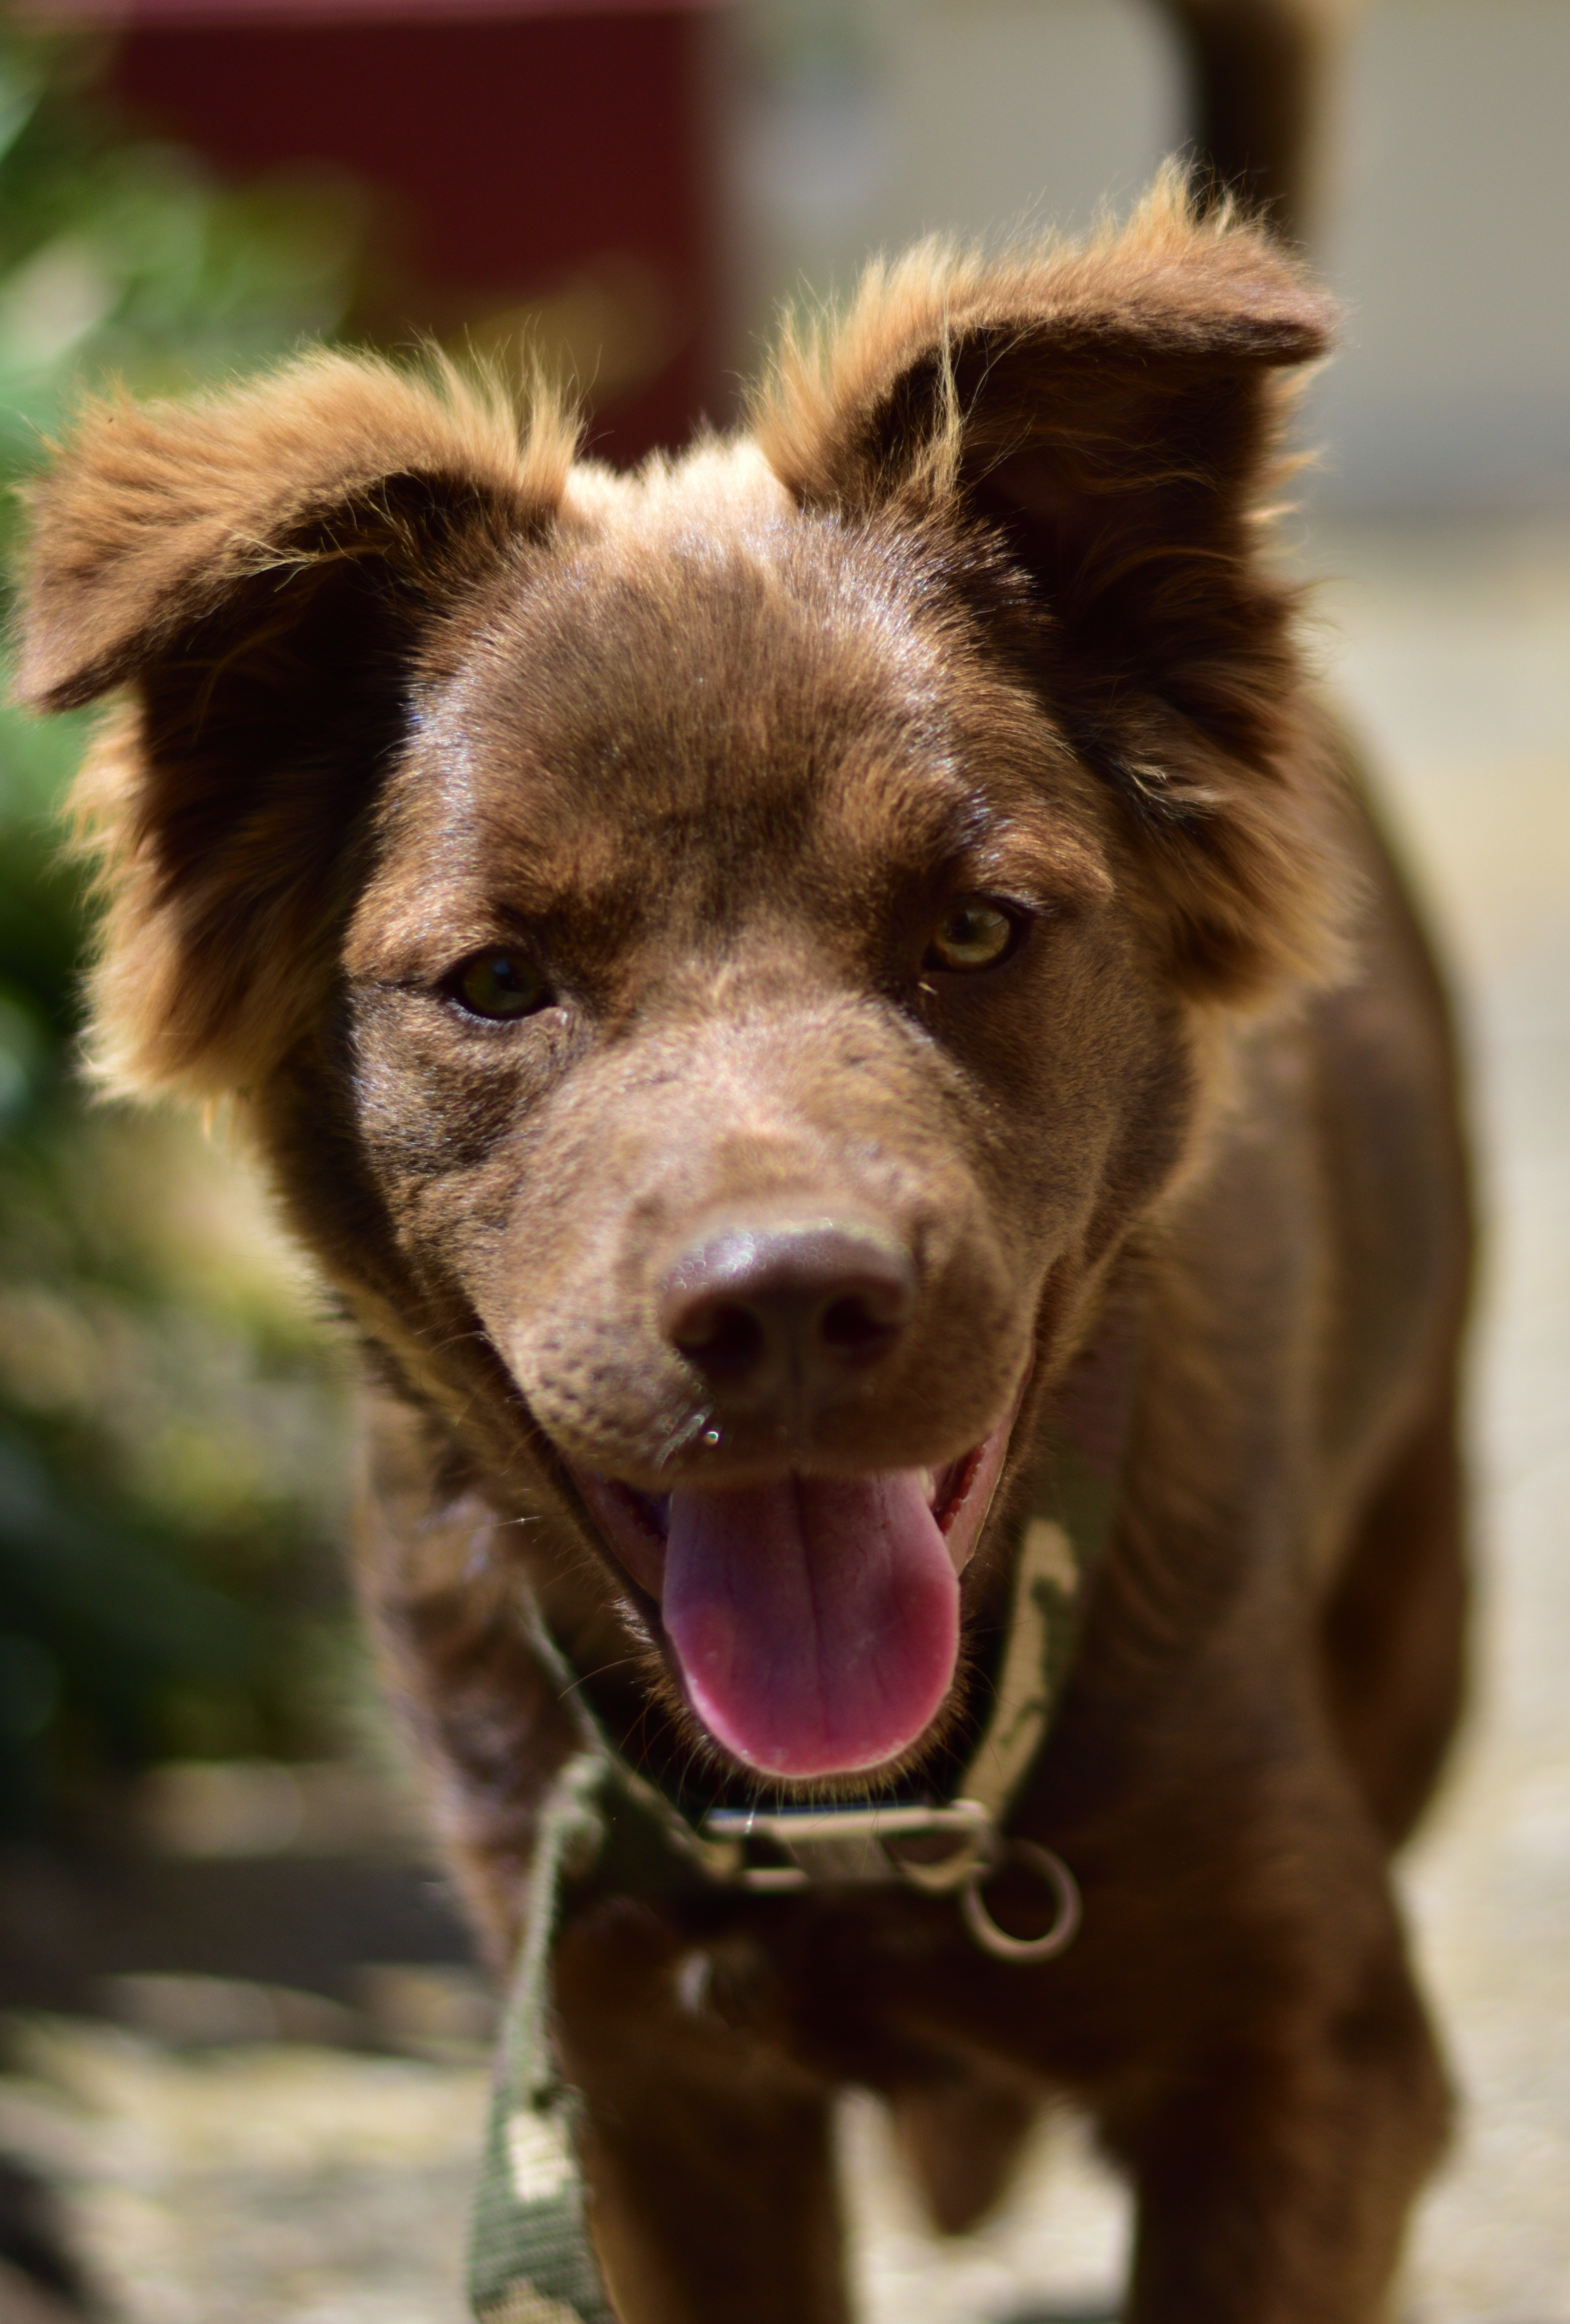
\includegraphics[width=0.5\textwidth]{resources/kep}
    \end{figure}
    \blindtext[5]
    \section{Fontok, betűk}
        \subsection{Alak}
            \textup{Álló karakterek} %upshape
            \textsl{Döntött} %slshape
            \textit{kurzív}  %itshape
            \textsc{Kiskapitális} %scshape
            {
                \itshape
                Csak ezt szedd Rekurzív karakterekkel
            }

        \subsection{Vastagság}
            \textmd{Normál} %mdseries
            \textbf{Félkövér} %bfseries
            {
                \bfseries
                Csak ez legyen Félkövér
            }
        \subsection{Család}
            \textrm{Antikva} %rmfamily
            \textsf{Sans serif} %sffamily
            \texttt{Írógép} %ttfamily
            {
                \ttfamily
                Csak ez legyen Írógép stílusu
            }
        \subsection{Méretek}
            \normalsize Normál
            \small Egyel kissebb
            \footnotesize Kettővel kissebb
            \scriptsize Hárommal kissebb
            \tiny Legkissebb

            \large Egyel nagyobb
            \Large Kettővel nagyobb
            \LARGE Hárommal nagyobb
            \huge Néggyel nagyobb
            \Huge Legnagyobb
            \begin{footnotesize}
                Ez egy lábjegyzet-méretű betűket tartalmazó blokk
            \end{footnotesize}
            Itt még mindig "Huge" a betűméret
            \emph{A kiemelés parancsa}
            {
                \em
                Ez pedig a kiemelést végző deklaráció
            }
            \underline{Aláhúzás}
            \uline{A jobbik aláhúzás}
            \uuline{Dupla aláhúzás}
            \uwave{Hullámos aláhúzás}
            \sout{Áthúzás}
            \xout{Kisatírozás}
            \MakeUppercase{Nagybetűs kiemelés}
            \MakeLowercase{Kis\-betű\-sí\-tés}
            \textnormal{Vissza a szokásos betűkhöz}
            De maradunk itt a Hugenál
            \normalsize\normalfont Innentől szokásos betűkkel dolgozunk
        \subsection{Verbatim Szövegek}
            \verb|Ez    egy verbatim   szöveg &\Ä|
            \verb*|Ez    egy visszajelzett verbatim   szöveg &\Ä|
            \begin{verbatim}
                Ez is    egy verbatim   szöveg &\Ä
            \end{verbatim}
            \lstinline|A=zeros(N,1);|
            \begin{lstlisting}[language=LaTex]
\documentclass[]{article}
%Ez itt a preambulum
\usepackage[utf8]{inputenc}
\usepackage[T1]{fontenc}
\usepackage{times}
\usepackage{blindtext}
\usepackage[margin=1.5in]{geometry}
\begin{document}
	\textit{Szevasz} \textbf{világ} $\sqrt(2)$
	 $$\sqrt(2)$$
	 \'a \'e \'W
	 \"o
	 \H{o}
	 \ss
	 \~n
	 \o
	 \underline{aláhúzott}
	\textbackslash
	\begin{equation}
		a_1^2+a_2^2=a_3^2\label{eq:equation}
	\end{equation}
	\begin{eqnarray}
		a_1^2+a_2^2&=&a_3^2\\
		a_1^2+a_2^2&=&a_3^2
	\end{eqnarray}
	\iffalse
	Ez a rész egy komment
	és többsoros.
	\fi
	\begin{flushleft}
		\blindtext
	\end{flushleft}
	\begin{center}
		\blindtext
	\end{center}
	szó  szó                    szó
	Új bekezdés \par
	Ez is új bekezdés\\
	Ez új sor \newline
	Ez is új sor \linebreak
	itt volt egy sortörés
	\begin{itemize}
		\item Számozatlan
		\item Lista
	\end{itemize}
	\begin{enumerate}
		\item Számozott
		\item Lista
		\item[69] Élem
	\end{enumerate}
	\begin{table}
		\caption{Táblázat címe}
		\begin{tabular}{|l||cr|}
			E&R&T\\ \hline
			EEE&RRR&TTT\\ \hline
		\end{tabular}\label{tab:table}
	\end{table}
	\'a^3
\end{document}

            \end{lstlisting}
            \begin{minted}{c}
                int main()
                {
                    printf("Hello World");
                    return 0;
                }
            \end{minted}
            \fontsize{14pt}{21pt}\selectfont
            \blindtext
            \usefont{T1}{ptm}{b}{it}\selectfont
            \blindtext
            \begin{flushleft}
                \blindtext
            \end{flushleft}
            \begin{flushright}
                \blindtext
            \end{flushright}
        \subsection{boxok}

\end{document}